\documentclass{article}

\title{Title}
\author{Author}
\date{Date}

\usepackage{amsmath}
\usepackage{graphicx}
\usepackage{natbib}

\begin{document}
\maketitle

\begin{abstract}
	Abstract
\end{abstract}

\section{Section one}
\label{s1}
Section \ref{s1} $\ldots$

Equation \eqref{e1} $\ldots$
\begin{align}
	\exp\left(i\pi\right)+1 & =0
	\label{e1}
\end{align}

Figure \ref{f1} $\ldots$
\begin{figure}
	\centering
	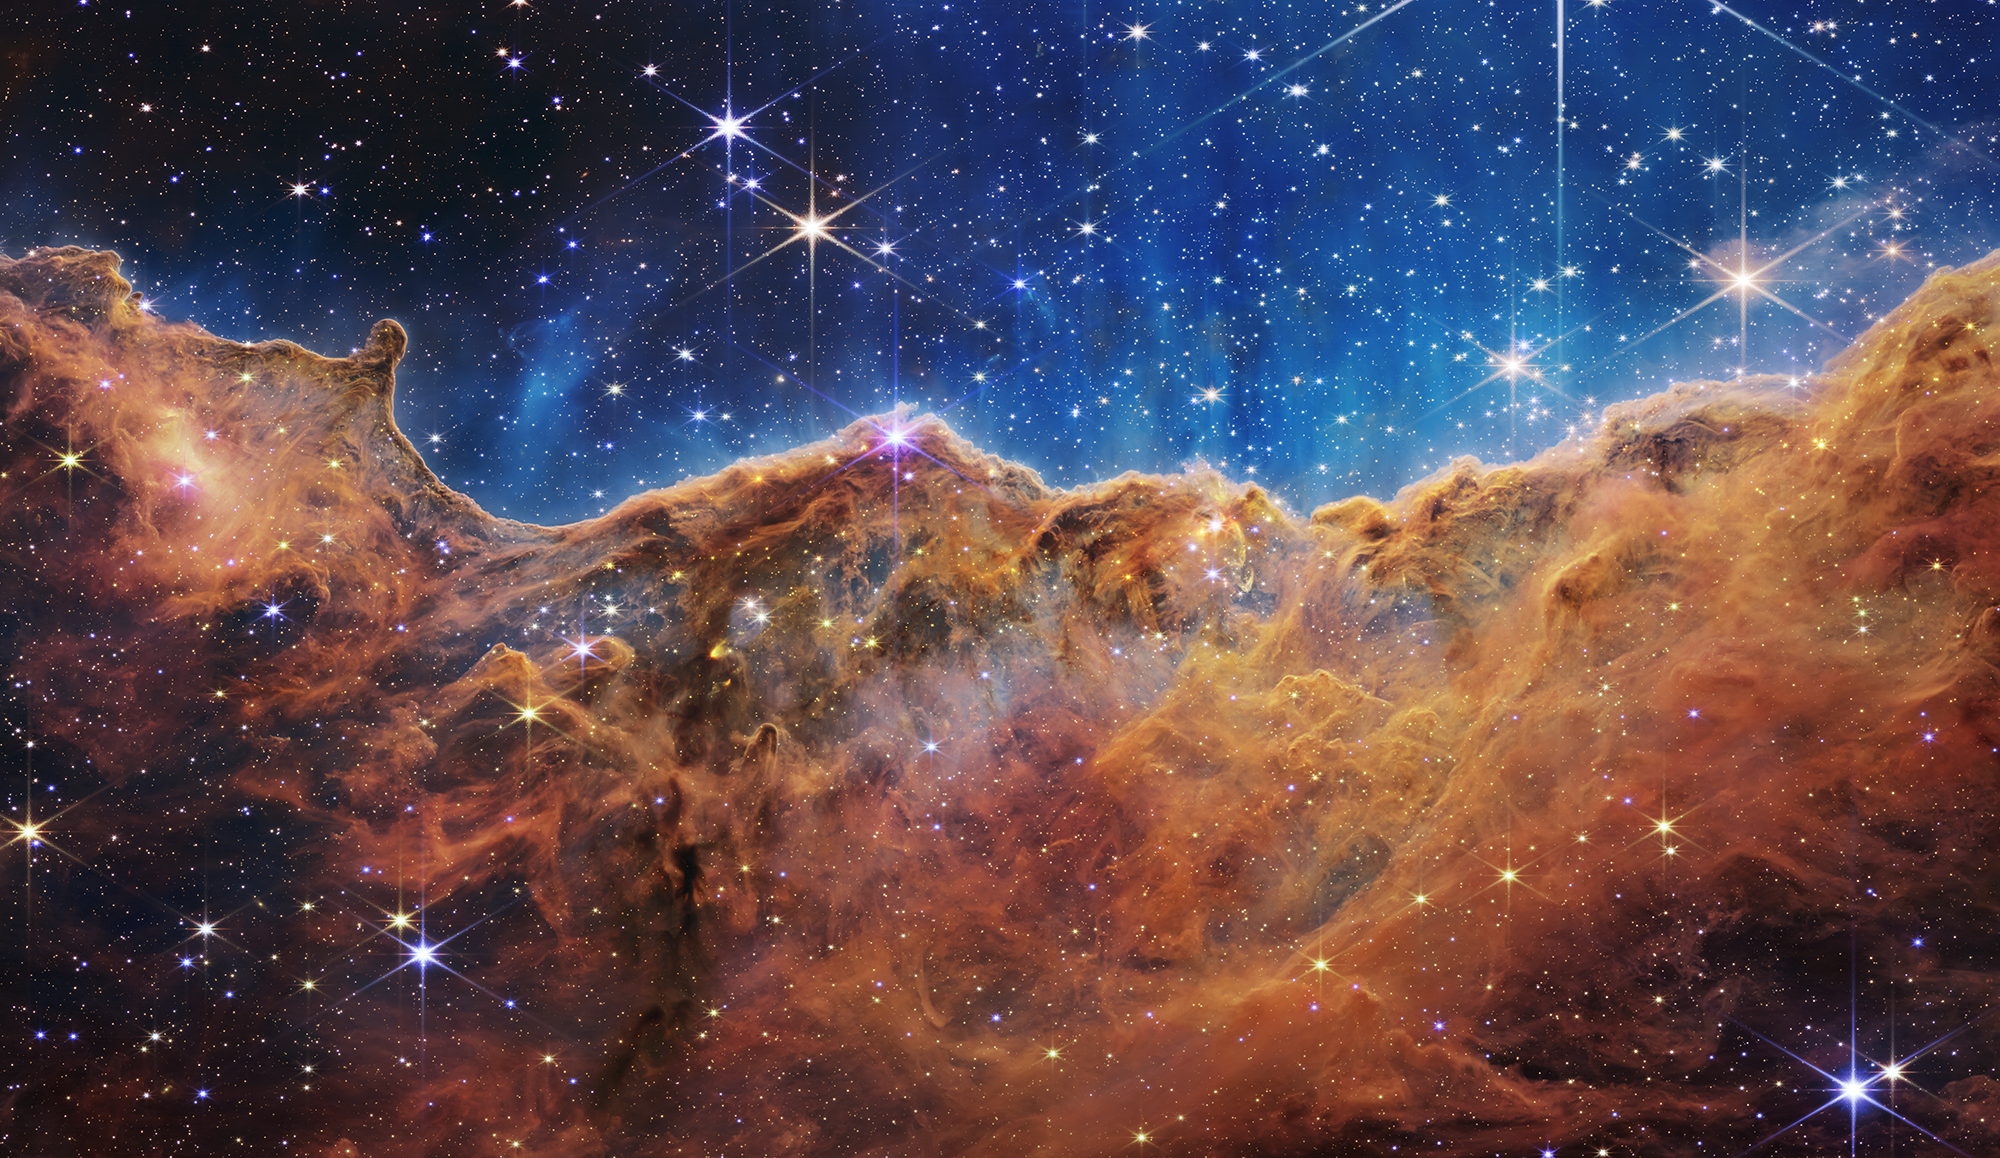
\includegraphics[width=0.7\linewidth]{2022090124bd9f962f9b894dc131a333eaa4c91c31ab71499b40f9d8f48ff56abcf96458/nasas-webb-reveals-cosmic-cliffs-glittering-landscape-of-star-birth_52211883534_o}
	\caption{Caption}
	\label{f1}
\end{figure}

\citet{Thomas2018} $\ldots$

\section{Principal component analysis}

\begin{align}
	\mathcal{L} & =\frac{1}{n-1}\sum_{i=1}^{n}\left(\hat{\mathbf{u}}_{1}^{T}\mathbf{x}_{i}-\hat{\mathbf{u}}_{1}^{T}\bar{\mathbf{x}}\right)\left(\hat{\mathbf{u}}_{1}^{T}\mathbf{x}_{i}-\hat{\mathbf{u}}_{1}^{T}\bar{\mathbf{x}}\right)^{T}-\lambda\left(\hat{\mathbf{u}}_{1}^{T}\hat{\mathbf{u}}_{1}-1\right)\\
	& =\hat{\mathbf{u}}_{1}^{T}\left(\frac{1}{n-1}\sum_{i=1}^{n}\left(\mathbf{x}_{i}-\bar{\mathbf{x}}\right)\left(\mathbf{x}_{i}-\bar{\mathbf{x}}\right)^{T}\right)\hat{\mathbf{u}}_{1}-\lambda\left(\hat{\mathbf{u}}_{1}^{T}\hat{\mathbf{u}}_{1}-1\right)\\
	& =\hat{\mathbf{u}}_{1}^{T}\mathbf{S}\hat{\mathbf{u}}_{1}-\lambda\left(\hat{\mathbf{u}}_{1}^{T}\hat{\mathbf{u}}_{1}-1\right)
\end{align}

\subsection{Projection}

\begin{align}
	\hat{\mathbf{u}} & =\frac{\mathbf{u}}{\left|\mathbf{u}\right|}
\end{align}

\begin{align}
	\textrm{proj}_{\hat{\mathbf{u}}}\mathbf{x} & =c\hat{\mathbf{u}}
\end{align}

\begin{align}
	c & =\left\langle \hat{\mathbf{u}},\mathbf{x}\right\rangle 
\end{align}

\begin{align}
	\textrm{proj}_{\hat{\mathbf{u}}}\mathbf{x} & =\left\langle \hat{\mathbf{u}},\mathbf{x}\right\rangle \hat{\mathbf{u}}
\end{align}

\subsection{Covariance}

\subsubsection{Univariate}

\begin{align}
	\sigma^{2} & =E\left(x-E\left(x\right)\right)^{2}
\end{align}

\begin{align}
	s^{2} & =\frac{1}{n-1}\sum_{i=1}^{n}\left(x_{i}-\bar{x}\right)^{2}
\end{align}

\subsubsection{Multivariate}

\begin{align}
	\mathbf{\Sigma} & =E\left[\begin{array}{cc}
		\left(x_{1}-E\left(x_{1}\right)\right)^{2} & \left(x_{1}-E\left(x_{1}\right)\right)\left(x_{2}-E\left(x_{2}\right)\right)\\
		\left(x_{2}-E\left(x_{2}\right)\right)\left(x_{1}-E\left(x_{1}\right)\right) & \left(x_{2}-E\left(x_{2}\right)\right)^{2}
	\end{array}\right]\\
	& =E\left[\begin{array}{c}
		x_{1}-E\left(x_{1}\right)\\
		x_{2}-E\left(x_{2}\right)
	\end{array}\right]\left[\begin{array}{cc}
		x_{1}-E\left(x_{1}\right) & x_{2}-E\left(x_{2}\right)\end{array}\right]\\
	& =E\left(\mathbf{x}-E\left(\mathbf{x}\right)\right)\left(\mathbf{x}-E\left(\mathbf{x}\right)\right)^{T}
\end{align}

\begin{align}
	\mathbf{S} & =\frac{1}{n-1}\sum_{i=1}^{n}\left[\begin{array}{cc}
		\left(x_{i,1}-\bar{x}_{1}\right)^{2} & \left(x_{i,1}-\bar{x}_{1}\right)\left(x_{i,2}-\bar{x}_{2}\right)\\
		\left(x_{i,2}-\bar{x}_{2}\right)\left(x_{i,1}-\bar{x}_{1}\right) & \left(x_{i,2}-\bar{x}_{2}\right)^{2}
	\end{array}\right]\\
	& =\frac{1}{n-1}\sum_{i=1}^{n}\left[\begin{array}{c}
		x_{i,1}-\bar{x}_{1}\\
		x_{i,2}-\bar{x}_{2}
	\end{array}\right]\left[\begin{array}{cc}
		x_{i,1}-\bar{x}_{1} & x_{i,2}-\bar{x}_{2}\end{array}\right]\\
	& =\frac{1}{n-1}\sum_{i=1}^{n}\left(\mathbf{x}_{i}-\bar{\mathbf{x}}\right)\left(\mathbf{x}_{i}-\bar{\mathbf{x}}\right)^{T}
\end{align}

\subsection{Lagragian}

\subsection{Derivative}

\subsection{Decomposition}

\begin{align}
	\mathbf{A}\mathbf{v}_{1} & =\lambda_{1}\mathbf{v}_{1}\\
	\mathbf{A}\mathbf{v}_{2} & =\lambda_{2}\mathbf{v}_{2}
\end{align}

\begin{align}
	\mathbf{A}\left[\begin{array}{cc}
		\mathbf{v}_{1} & \mathbf{v}_{2}\end{array}\right] & =\left[\begin{array}{cc}
		\mathbf{v}_{1} & \mathbf{v}_{2}\end{array}\right]\left[\begin{array}{cc}
		\lambda_{1} & 0\\
		0 & \lambda_{2}
	\end{array}\right]
\end{align}

\begin{align}
	\mathbf{A}\mathbf{V} & =\mathbf{V}\mathbf{\Lambda}
\end{align}

\begin{align}
	\mathbf{A} & =\mathbf{V}\mathbf{\Lambda}\mathbf{V}^{-1}
\end{align}

\section{Latent semantic analysis}

\subsection{Decomposition}

\begin{align}
	\mathbf{B} & =\sigma_{1}\mathbf{u}_{1}\mathbf{v}_{1}^{T}+\sigma_{2}\mathbf{u}_{2}\mathbf{v}_{2}^{T}
\end{align}

\begin{align}
	\mathbf{B} & =\left[\begin{array}{cc}
		\mathbf{u}_{1} & \mathbf{u}_{2}\end{array}\right]\left[\begin{array}{cc}
		\sigma_{1} & 0\\
		0 & \sigma_{2}
	\end{array}\right]\left[\begin{array}{c}
		\mathbf{v}_{1}^{T}\\
		\mathbf{v}_{2}^{T}
	\end{array}\right]
\end{align}

\begin{align}
	\mathbf{B} & =\mathbf{U}\mathbf{\Sigma}\mathbf{V}^{T}
\end{align}

\begin{align}
	\mathbf{B}\mathbf{V} & =\mathbf{U}\mathbf{\Sigma}
\end{align}

\bibliography{draft}
\bibliographystyle{agsm}
\end{document}